% 1977 年江苏苏州地区初试卷第三题（4）小题：AB 为半圆的直径，CD⊥AB 于 D，C 在圆上（按源卷第1页布局）
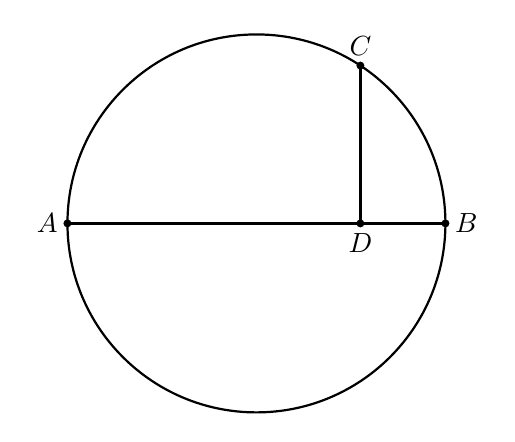
\begin{tikzpicture}[scale=1.2]
  \coordinate (O) at (0,0);
  \coordinate (A) at (-2,0);
  \coordinate (B) at (2,0);
  \coordinate (D) at (1.1,0);
  \coordinate (C) at (1.1,1.67);
  \draw[thick] (O) circle (2);
  \draw[thick] (A)--(B);
  \draw[thick] (C)--(D);
  \fill (A) circle (1.2pt) node[left] {$A$};
  \fill (B) circle (1.2pt) node[right] {$B$};
  \fill (C) circle (1.2pt) node[above] {$C$};
  \fill (D) circle (1.2pt) node[below] {$D$};
\end{tikzpicture}
